% ============================================================
%  L02_mini5.tex  --  Fintech Ecosystem
%  5-Slide Teaser Arc: WHY > WHAT > HOW > WHERE > SO WHAT
%  Self-contained (no \input{} commands, no \includegraphics)
%  Compile: pdflatex L02_mini5.tex  (twice for overlays)
% ============================================================

\documentclass[aspectratio=169, 11pt]{beamer}
\usetheme{Madrid}
\usecolortheme{whale}
\usepackage{tikz,pgfplots,booktabs,multicol,amsmath}
\usetikzlibrary{arrows.meta,positioning,shapes.geometric,calc,decorations.pathmorphing}
\pgfplotsset{compat=1.18}

% ---- Colour palette ----------------------------------------
\definecolor{mlpurple}{HTML}{9467BD}
\definecolor{mlblue}{HTML}{1F77B4}
\definecolor{mlred}{HTML}{D62728}
\definecolor{mlorange}{HTML}{FF7F0E}
\definecolor{mlgreen}{HTML}{2CA02C}
\definecolor{mlgray}{HTML}{7F7F7F}
\definecolor{mlteal}{HTML}{0D7377}
\definecolor{mlcyan}{HTML}{14BDEB}

% ---- Beamer theme colours ----------------------------------
\setbeamercolor{structure}{fg=mlteal}
\setbeamercolor{palette primary}{bg=mlteal,fg=white}
\setbeamercolor{palette secondary}{bg=mlteal!80,fg=white}
\setbeamercolor{palette tertiary}{bg=mlteal!60,fg=white}
\setbeamercolor{frametitle}{bg=mlteal!10,fg=mlteal}
\setbeamercolor{title}{fg=white}
\setbeamercolor{subtitle}{fg=mlcyan!80}
\setbeamercolor{block title}{bg=mlteal,fg=white}
\setbeamercolor{block body}{bg=mlteal!8,fg=black}
\setbeamercolor{block title alerted}{bg=mlred!80,fg=white}
\setbeamercolor{block body alerted}{bg=mlred!8,fg=black}

% ---- Bottom-note command -----------------------------------
\newcommand{\bottomnote}[1]{%
  \vfill
  \begin{beamercolorbox}[wd=\textwidth,ht=2ex,dp=1ex]{palette primary}%
    \tiny\hspace{1em}#1%
  \end{beamercolorbox}}

% ---- Metadata ----------------------------------------------
\title{Fintech Ecosystem}
\subtitle{5-Slide Teaser}
\author{Joerg Osterrieder}
\institute{University of Zurich}
\date{Spring 2026}
\setbeamertemplate{navigation symbols}{}

% ============================================================
\begin{document}
% ============================================================

% -----------------------------------------------------------
%  TITLE FRAME (not counted in the 5)
% -----------------------------------------------------------
\begin{frame}
  \titlepage
  \bottomnote{Financial Technology (FinTech) -- MSc Course | University of Zurich | Spring 2026}
\end{frame}

% ===========================================================
%  SLIDE 1 of 5  --  WHY
%  Visual: TikZ comic -- farmer with phone, closed bank branch
% ===========================================================
\begin{frame}{Why Fintech? The Unbanked Get a Signal}

\begin{center}
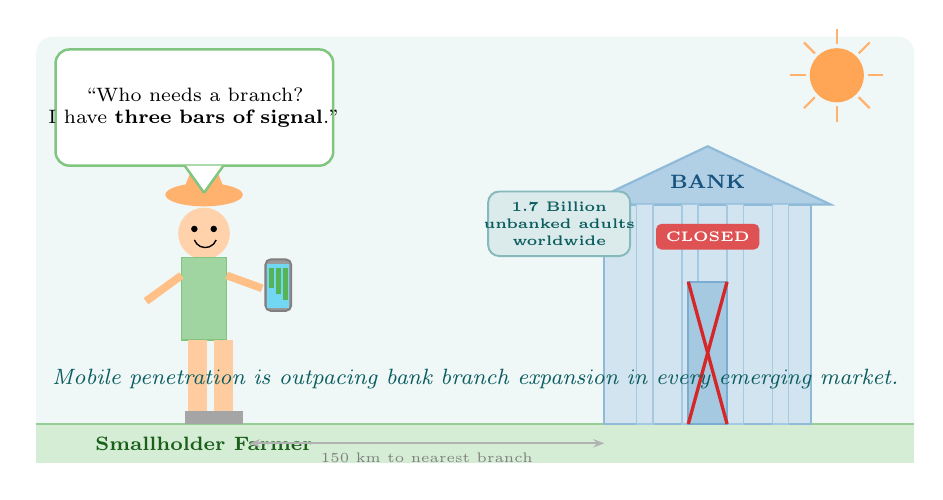
\begin{tikzpicture}[scale=0.82, every node/.style={font=\small}]

  % ---- Background strip ----
  \fill[mlteal!6, rounded corners=6pt] (-6.8,-2.8) rectangle (6.8,3.8);

  % ---- Ground line ----
  \fill[mlgreen!20] (-6.8,-2.8) rectangle (6.8,-2.2);
  \draw[mlgreen!50, line width=0.6pt] (-6.8,-2.2) -- (6.8,-2.2);

  % ---- SUN (top right) ----
  \fill[mlorange!70] (5.6,3.2) circle (0.42);
  \foreach \a in {0,45,90,135,180,225,270,315}{
    \draw[mlorange!60, line width=0.8pt]
      ({5.6+0.48*cos(\a)},{3.2+0.48*sin(\a)}) --
      ({5.6+0.72*cos(\a)},{3.2+0.72*sin(\a)});
  }

  % ---- CLOSED BANK BRANCH (right side) ----
  % Building body
  \fill[mlblue!20, draw=mlblue!50, line width=0.8pt]
    (2.0,-2.2) rectangle (5.2,1.2);
  % Roof / pediment
  \fill[mlblue!35, draw=mlblue!50, line width=0.8pt]
    (1.7,1.2) -- (5.5,1.2) -- (3.6,2.1) -- cycle;
  % Columns
  \foreach \cx in {2.5, 3.2, 3.9, 4.6}{
    \fill[white!80!mlblue, draw=mlblue!40, line width=0.5pt]
      (\cx,-2.2) rectangle (\cx+0.25,1.2);
  }
  % Door (closed, crossed out)
  \fill[mlblue!40, draw=mlblue!60, line width=0.6pt]
    (3.3,-2.2) rectangle (3.9,0.0);
  \draw[mlred, line width=1.2pt] (3.3,-2.2) -- (3.9,0.0);
  \draw[mlred, line width=1.2pt] (3.9,-2.2) -- (3.3,0.0);
  % "CLOSED" sign
  \fill[mlred!80, rounded corners=2pt]
    (2.8,0.5) rectangle (4.4,0.9);
  \node[font=\tiny\bfseries, text=white] at (3.6,0.7) {CLOSED};
  % Bank label
  \node[font=\scriptsize\bfseries, text=mlblue!70!black] at (3.6,1.55) {BANK};

  % ---- FARMER FIGURE (left side) ----
  % Hat
  \fill[mlorange!60] (-4.2,1.35) ellipse (0.6 and 0.18);
  \fill[mlorange!50] (-4.2,1.35) rectangle (-4.2,1.72);
  \fill[mlorange!60] (-4.55,1.35) -- (-3.85,1.35) -- (-4.0,1.72) -- (-4.4,1.72) -- cycle;
  % Head
  \fill[mlorange!35] (-4.2,0.75) circle (0.40);
  % Eyes
  \fill[black] (-4.35,0.82) circle (0.05);
  \fill[black] (-4.05,0.82) circle (0.05);
  % Smile
  \draw[black, line width=0.5pt] (-4.35,0.65) arc(200:340:0.18);
  % Body (shirt)
  \fill[mlgreen!45, draw=mlgreen!60, line width=0.6pt]
    (-4.55,-0.9) rectangle (-3.85,0.38);
  % Arms
  \draw[mlorange!50, line width=2.8pt] (-4.55,0.1) -- (-5.1,-0.3);
  % Right arm holding phone
  \draw[mlorange!50, line width=2.8pt] (-3.85,0.1) -- (-3.3,-0.1);
  % PHONE in right hand
  \fill[mlgray!80, draw=mlgray, line width=0.7pt, rounded corners=2pt]
    (-3.25,-0.45) rectangle (-2.85,0.35);
  \fill[mlcyan!60] (-3.22,-0.40) rectangle (-2.88,0.28);
  % Signal bars on phone screen
  \fill[mlgreen!80] (-3.20,-0.10) rectangle (-3.12,0.22);
  \fill[mlgreen!80] (-3.09,-0.18) rectangle (-3.01,0.22);
  \fill[mlgreen!80] (-2.98,-0.28) rectangle (-2.90,0.22);
  % Legs
  \fill[mlorange!40] (-4.45,-0.9) rectangle (-4.15,-2.0);
  \fill[mlorange!40] (-4.05,-0.9) rectangle (-3.75,-2.0);
  % Boots
  \fill[mlgray!70] (-4.5,-2.0) rectangle (-4.0,-2.2);
  \fill[mlgray!70] (-4.1,-2.0) rectangle (-3.6,-2.2);
  % Farmer label
  \node[mlgreen!60!black, font=\scriptsize\bfseries] at (-4.2,-2.5) {Smallholder Farmer};

  % ---- SPEECH BUBBLE from farmer ----
  \fill[white, rounded corners=5pt]
    (-6.5,1.8) rectangle (-2.2,3.6);
  \draw[mlgreen!60, rounded corners=5pt, line width=0.9pt]
    (-6.5,1.8) rectangle (-2.2,3.6);
  % Bubble tail toward farmer head
  \fill[white] (-4.5,1.8) -- (-4.2,1.38) -- (-3.9,1.8) -- cycle;
  \draw[mlgreen!60, line width=0.9pt] (-4.5,1.8) -- (-4.2,1.38);
  \draw[mlgreen!60, line width=0.9pt] (-4.2,1.38) -- (-3.9,1.8);
  \node[align=center, font=\scriptsize, text width=4.0cm]
    at (-4.35,2.7)
    {``Who needs a branch?\\I have \textbf{three bars of signal}.''};

  % ---- Distance arrow from farmer to bank ----
  \draw[mlgray!60, {Stealth[length=4pt]}-{Stealth[length=4pt]}, line width=0.7pt]
    (-3.5,-2.5) -- (2.0,-2.5);
  \node[font=\tiny, mlgray] at (-0.75,-2.72) {150 km to nearest branch};

  % ---- 1.7B callout (centre-right area) ----
  \fill[mlteal!15, rounded corners=4pt, draw=mlteal!50, line width=0.7pt]
    (0.2,0.4) rectangle (2.4,1.4);
  \node[align=center, font=\tiny\bfseries, text=mlteal!80!black]
    at (1.3,0.9) {\textbf{1.7 Billion}\\unbanked adults\\worldwide};

  % ---- Caption ----
  \node[mlteal!80!black, font=\footnotesize\itshape, align=center]
    at (0,-1.5)
    {Mobile penetration is outpacing bank branch expansion in every emerging market.};

\end{tikzpicture}
\end{center}

\bottomnote{Slide 1/5 -- WHY | 1.7B unbanked adults; mobile subscriptions exceed bank accounts globally (GSMA 2024, World Bank Findex).}
\end{frame}

% ===========================================================
%  SLIDE 2 of 5  --  WHAT
%  Visual: booktabs table -- growth drivers + inclusion gap
% ===========================================================
\begin{frame}[shrink=5]{What Drives the Fintech Ecosystem?}

\vspace{-0.3em}
\begin{columns}[T]
\begin{column}{0.55\textwidth}

  \textcolor{mlteal}{\textbf{\small Four Growth Driver Groups}}
  \vspace{0.4em}

  \scriptsize
  \setlength{\tabcolsep}{4pt}
  \renewcommand{\arraystretch}{1.22}
  \begin{tabular}{@{}p{2.6cm}p{2.4cm}l@{}}
    \toprule
    \textbf{Driver} & \textbf{Mechanism} & \textbf{Signal} \\
    \midrule
    \textbf{Technology} & Smartphone + cloud & 6.9B subscriptions \\
    \textbf{Regulation} & PSD2, open banking & 50+ sandbox regimes \\
    \textbf{Capital} & VC \& PE inflows & \$226B (2021 peak) \\
    \textbf{Demographics} & Digital-native users & 72\% prefer mobile \\
    \bottomrule
  \end{tabular}

  \vspace{0.5em}
  \begin{block}{Ecosystem Definition}
    \scriptsize
    The fintech \emph{ecosystem} = startups, incumbents, BigTech,
    regulators, investors, and infrastructure providers -- all
    \textbf{co-evolving} around digital finance.
  \end{block}

\end{column}
\begin{column}{0.42\textwidth}
  \vspace{0.1em}
  \textcolor{mlred}{\textbf{\small The Inclusion Gap}}
  \vspace{0.3em}

  \begin{itemize}\scriptsize
    \setlength{\itemsep}{3pt}
    \item[\textcolor{mlred}{$\blacktriangleright$}]
      \textbf{1.7B adults} lack a bank account
    \item[\textcolor{mlorange}{$\blacktriangleright$}]
      \textbf{Cost} is the \#1 stated barrier (World Bank)
    \item[\textcolor{mlorange}{$\blacktriangleright$}]
      \textbf{Distance} \& documentation close second
    \item[\textcolor{mlgreen}{$\blacktriangleright$}]
      Mobile money \textbf{bridges the gap}: M-Pesa, bKash, UPI
    \item[\textcolor{mlgreen}{$\blacktriangleright$}]
      Fintech can deliver credit scoring \textbf{without credit history}
    \item[\textcolor{mlteal}{$\blacktriangleright$}]
      Regulators shift from \emph{``no''} to \emph{``sandbox first''}
  \end{itemize}

  \vspace{0.4em}
  \begin{alertblock}{\scriptsize Key Tension}
    \tiny
    Growth is fastest where traditional banking is
    \textbf{weakest} -- but so is consumer protection infrastructure.
  \end{alertblock}
\end{column}
\end{columns}

\bottomnote{Slide 2/5 -- WHAT | Ecosystem thinking: no single actor dominates -- value emerges from interactions across layers.}
\end{frame}

% ===========================================================
%  SLIDE 3 of 5  --  HOW
%  Visual: TikZ architecture -- choice architecture / nudge framework
% ===========================================================
\begin{frame}{How Does Fintech Shape Behaviour? Choice Architecture}

\begin{center}
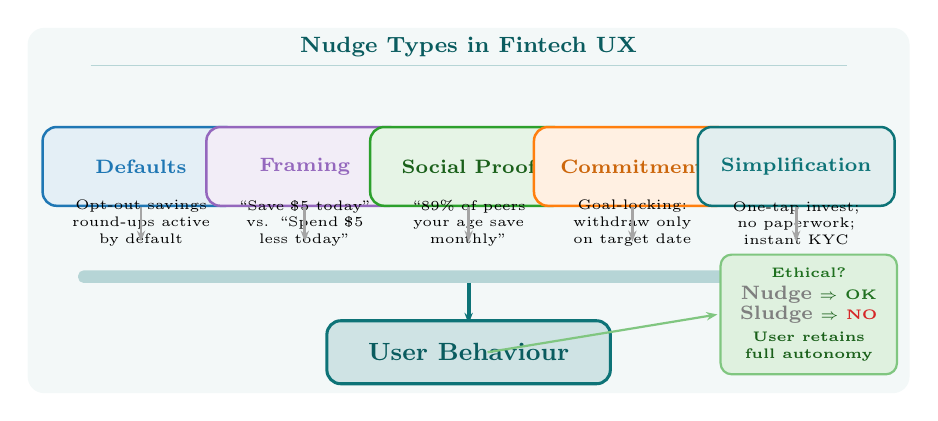
\begin{tikzpicture}[
    scale=0.80,
    nudge/.style={rectangle, rounded corners=5pt, minimum width=2.5cm,
                  minimum height=1.0cm, align=center, font=\scriptsize\bfseries,
                  line width=0.9pt, draw},
    arr/.style={-{Stealth[length=4pt]}, line width=1.0pt},
    every node/.style={font=\small}
  ]

  % ---- Background ----
  \fill[mlteal!5, rounded corners=6pt] (-7.0,-2.8) rectangle (7.0,3.0);

  % ---- Title row ----
  \node[font=\footnotesize\bfseries, text=mlteal!80!black] at (0,2.7)
    {Nudge Types in Fintech UX};
  \draw[mlteal!30, line width=0.5pt] (-6.0,2.4) -- (6.0,2.4);

  % ---- Five nudge boxes (arranged in a single row, slightly staggered) ----

  % Box 1: Defaults
  \node[nudge, fill=mlblue!12, draw=mlblue]
    (n1) at (-5.2,0.8) {\textcolor{mlblue}{Defaults}};
  \node[font=\tiny, align=center, text width=2.2cm] at (-5.2,-0.1)
    {Opt-out savings\\round-ups active\\by default};

  % Box 2: Framing
  \node[nudge, fill=mlpurple!12, draw=mlpurple]
    (n2) at (-2.6,0.8) {\textcolor{mlpurple}{Framing}};
  \node[font=\tiny, align=center, text width=2.2cm] at (-2.6,-0.1)
    {``Save \$5 today''\\vs. ``Spend \$5\\less today''};

  % Box 3: Social Proof
  \node[nudge, fill=mlgreen!12, draw=mlgreen]
    (n3) at (0.0,0.8) {\textcolor{mlgreen!60!black}{Social Proof}};
  \node[font=\tiny, align=center, text width=2.2cm] at (0.0,-0.1)
    {``89\% of peers\\your age save\\monthly''};

  % Box 4: Commitment
  \node[nudge, fill=mlorange!12, draw=mlorange]
    (n4) at (2.6,0.8) {\textcolor{mlorange!80!black}{Commitment}};
  \node[font=\tiny, align=center, text width=2.2cm] at (2.6,-0.1)
    {Goal-locking:\\withdraw only\\on target date};

  % Box 5: Simplification
  \node[nudge, fill=mlteal!12, draw=mlteal]
    (n5) at (5.2,0.8) {\textcolor{mlteal}{Simplification}};
  \node[font=\tiny, align=center, text width=2.2cm] at (5.2,-0.1)
    {One-tap invest;\\no paperwork;\\instant KYC};

  % ---- Arrows all pointing down to behavior outcome ----
  \foreach \n in {n1,n2,n3,n4,n5}{
    \draw[arr, mlgray!70] (\n.south) -- ++(0,-0.55);
  }

  % ---- Horizontal collector bar ----
  \fill[mlteal!30, rounded corners=2pt] (-6.2,-1.05) rectangle (6.2,-0.85);

  % ---- Arrow from bar to outcome ----
  \draw[arr, mlteal, line width=1.4pt] (0,-1.05) -- (0,-1.7);

  % ---- User Behavior outcome box ----
  \node[rectangle, rounded corners=5pt, fill=mlteal!20, draw=mlteal,
        minimum width=3.6cm, minimum height=0.8cm,
        font=\small\bfseries, line width=1.1pt]
    at (0,-2.15) {\textcolor{mlteal!80!black}{User Behaviour}};

  % ---- Ethical filter (right side annotation) ----
  \fill[mlgreen!15, draw=mlgreen!60, line width=0.8pt, rounded corners=4pt]
    (4.0,-2.5) rectangle (6.8,-0.6);
  \node[font=\tiny\bfseries, text=mlgreen!60!black, align=center]
    at (5.4,-1.55) {\textcolor{mlgreen!70!black}{Ethical?}\\[2pt]
    \textcolor{mlgray}{\scriptsize Nudge} $\Rightarrow$ \textcolor{mlgreen!70!black}{OK}\\
    \textcolor{mlgray}{\scriptsize Sludge} $\Rightarrow$ \textcolor{mlred}{\textbf{NO}}\\[2pt]
    \tiny User retains\\full autonomy};

  % ---- Arrow pointing to ethical box ----
  \draw[arr, mlgreen!60, line width=0.8pt] (0.3,-2.15) -- (3.95,-1.55);

\end{tikzpicture}
\end{center}

\bottomnote{Slide 3/5 -- HOW | Thaler \& Sunstein (2008): nudges preserve freedom of choice while improving outcomes -- fintech embeds this at scale.}
\end{frame}

% ===========================================================
%  SLIDE 4 of 5  --  WHERE
%  Visual: pgfplots grouped bar chart -- trust by provider type
% ===========================================================
\begin{frame}{Where Does Trust Sit? Comparing Provider Types}

\vspace{-0.3em}
\begin{center}
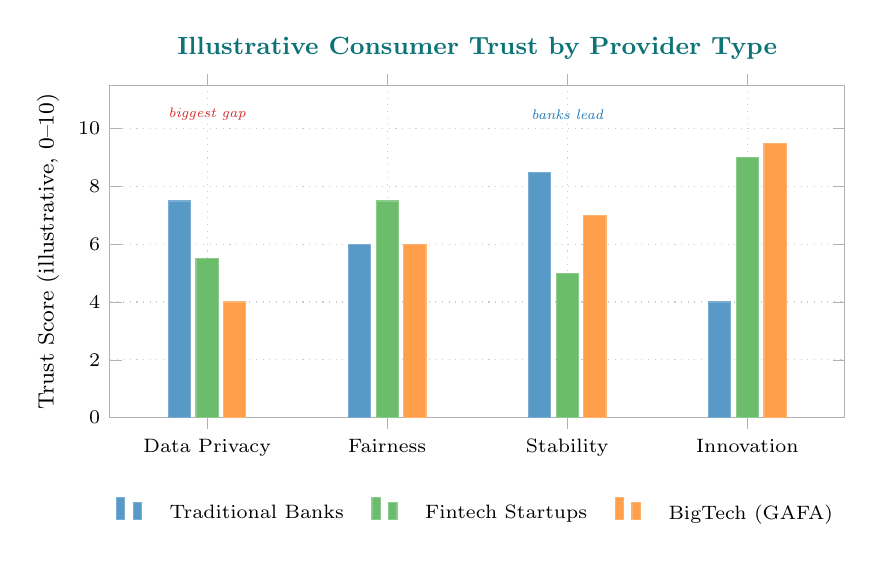
\begin{tikzpicture}
\begin{axis}[
    ybar,
    bar width=8pt,
    width=0.90\textwidth,
    height=5.8cm,
    enlarge x limits=0.18,
    ylabel={\footnotesize Trust Score (illustrative, 0--10)},
    ylabel style={font=\scriptsize},
    ymin=0, ymax=11.5,
    ytick={0,2,4,6,8,10},
    yticklabel style={font=\scriptsize},
    symbolic x coords={Data Privacy, Fairness, Stability, Innovation},
    xtick=data,
    xticklabel style={font=\scriptsize, align=center},
    legend style={
      at={(0.5,-0.22)},
      anchor=north,
      legend columns=3,
      font=\scriptsize,
      column sep=8pt,
      draw=none
    },
    legend cell align=left,
    grid=major,
    grid style={dotted, mlgray!40},
    axis line style={mlgray!60},
    tick style={mlgray!60},
    title={\small Illustrative Consumer Trust by Provider Type},
    title style={font=\small\bfseries, color=mlteal}
  ]

  % Traditional Banks
  \addplot[fill=mlblue!75, draw=mlblue!60] coordinates {
    (Data Privacy, 7.5)
    (Fairness,     6.0)
    (Stability,    8.5)
    (Innovation,   4.0)
  };

  % Fintech Startups
  \addplot[fill=mlgreen!70, draw=mlgreen!55] coordinates {
    (Data Privacy, 5.5)
    (Fairness,     7.5)
    (Stability,    5.0)
    (Innovation,   9.0)
  };

  % BigTech (GAFA)
  \addplot[fill=mlorange!75, draw=mlorange!60] coordinates {
    (Data Privacy, 4.0)
    (Fairness,     6.0)
    (Stability,    7.0)
    (Innovation,   9.5)
  };

  \legend{Traditional Banks, Fintech Startups, BigTech (GAFA)}

  % Annotation on Data Privacy
  \node[font=\tiny\itshape, text=mlred, align=center]
    at (axis cs:Data Privacy, 10.5) {biggest gap};

  % Annotation on Stability
  \node[font=\tiny\itshape, text=mlblue, align=center]
    at (axis cs:Stability, 10.5) {banks lead};

\end{axis}
\end{tikzpicture}
\end{center}
\vspace{-0.4em}
{\tiny\textcolor{mlgray}{\textit{Conceptual comparison -- illustrative scores. Actual trust varies by country, cohort, and product category.}}}

\bottomnote{Slide 4/5 -- WHERE | Trust is the scarce resource: banks own stability trust; fintechs own innovation trust; BigTech faces data-privacy deficit.}
\end{frame}

% ===========================================================
%  SLIDE 5 of 5  --  SO WHAT
%  Visual: TikZ 2x2 quadrant -- inclusion vs. protection trade-off
% ===========================================================
\begin{frame}{So What? Navigating the Inclusion--Protection Trade-Off}

\begin{center}
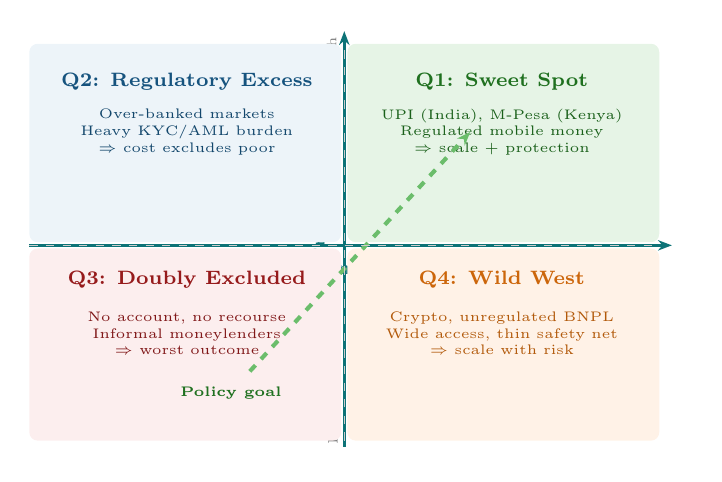
\begin{tikzpicture}[scale=0.80, every node/.style={font=\small}]

  % ---- Axes ----
  % X-axis: Financial Inclusion (left=low, right=high)
  \draw[mlteal, -{Stealth[length=5pt]}, line width=1.2pt] (-5.0,0) -- (5.2,0);
  \node[font=\scriptsize\bfseries, text=mlteal] at (5.4,0) {};
  \node[font=\scriptsize, text=mlteal, align=center] at (0,-0.35)
    {\textbf{Financial Inclusion} $\longrightarrow$};

  % Y-axis: Consumer Protection (bottom=low, top=high)
  \draw[mlteal, -{Stealth[length=5pt]}, line width=1.2pt] (0,-3.2) -- (0,3.4);
  \node[font=\scriptsize, text=mlteal, align=center, rotate=90] at (-0.42,0)
    {\textbf{Consumer Protection} $\longrightarrow$};

  % Axis end labels
  \node[font=\tiny, text=mlgray] at (-4.6,-0.2) {Low};
  \node[font=\tiny, text=mlgray] at (4.6,-0.2) {High};
  \node[font=\tiny, text=mlgray, rotate=90] at (-0.18,3.0) {High};
  \node[font=\tiny, text=mlgray, rotate=90] at (-0.18,-2.9) {Low};

  % ---- Quadrant backgrounds ----
  % Q2: top-left -- High protection, Low inclusion (Regulatory excess)
  \fill[mlblue!8, rounded corners=3pt] (-5.0,0.05) rectangle (-0.05,3.2);
  % Q1: top-right -- High-High (Sweet spot)
  \fill[mlgreen!12, rounded corners=3pt] (0.05,0.05) rectangle (5.0,3.2);
  % Q3: bottom-left -- Low-Low (Excluded and exposed)
  \fill[mlred!8, rounded corners=3pt] (-5.0,-3.1) rectangle (-0.05,-0.05);
  % Q4: bottom-right -- High inclusion, Low protection (Wild west)
  \fill[mlorange!10, rounded corners=3pt] (0.05,-3.1) rectangle (5.0,-0.05);

  % ---- Quadrant labels ----
  % Q1 (top-right): Sweet spot
  \node[font=\scriptsize\bfseries, text=mlgreen!70!black, align=center]
    at (2.5,2.6) {Q1: Sweet Spot};
  \node[font=\tiny, text=mlgreen!60!black, align=center, text width=4.0cm]
    at (2.5,1.8)
    {UPI (India), M-Pesa (Kenya)\\Regulated mobile money\\$\Rightarrow$ scale + protection};

  % Q2 (top-left): Regulatory excess
  \node[font=\scriptsize\bfseries, text=mlblue!70!black, align=center]
    at (-2.5,2.6) {Q2: Regulatory Excess};
  \node[font=\tiny, text=mlblue!60!black, align=center, text width=3.8cm]
    at (-2.5,1.8)
    {Over-banked markets\\Heavy KYC/AML burden\\$\Rightarrow$ cost excludes poor};

  % Q3 (bottom-left): Excluded and exposed
  \node[font=\scriptsize\bfseries, text=mlred!70!black, align=center]
    at (-2.5,-0.55) {Q3: Doubly Excluded};
  \node[font=\tiny, text=mlred!60!black, align=center, text width=3.8cm]
    at (-2.5,-1.4)
    {No account, no recourse\\Informal moneylenders\\$\Rightarrow$ worst outcome};

  % Q4 (bottom-right): Wild west
  \node[font=\scriptsize\bfseries, text=mlorange!80!black, align=center]
    at (2.5,-0.55) {Q4: Wild West};
  \node[font=\tiny, text=mlorange!70!black, align=center, text width=4.0cm]
    at (2.5,-1.4)
    {Crypto, unregulated BNPL\\Wide access, thin safety net\\$\Rightarrow$ scale with risk};

  % ---- Arrow pointing to Q1 ----
  \draw[mlgreen!70, -{Stealth[length=5pt]}, line width=1.5pt, dashed]
    (-1.5,-2.0) -- (2.0,1.8);
  \node[font=\tiny\bfseries, text=mlgreen!70!black, align=center]
    at (-1.8,-2.35) {Policy goal};

  % ---- Divider lines (axis) already drawn, reinforce with dashed ----
  \draw[mlgray!40, line width=0.4pt, dashed] (-5.0,0) -- (5.0,0);
  \draw[mlgray!40, line width=0.4pt, dashed] (0,-3.1) -- (0,3.2);

\end{tikzpicture}
\end{center}

\bottomnote{Slide 5/5 -- SO WHAT | The ecosystem's mandate: move every market toward Q1. Requires coordinated innovation, regulation, and trust-building.}
\end{frame}

% ===========================================================
%  END
% ===========================================================
\end{document}
